\chapter{Développements Logiciel : Conception, Modélisation, Implémentation} 

\section{Développements logiciel}

\section{Modules}

\begin{figure}[!htbp]
\center
	\subfloat{{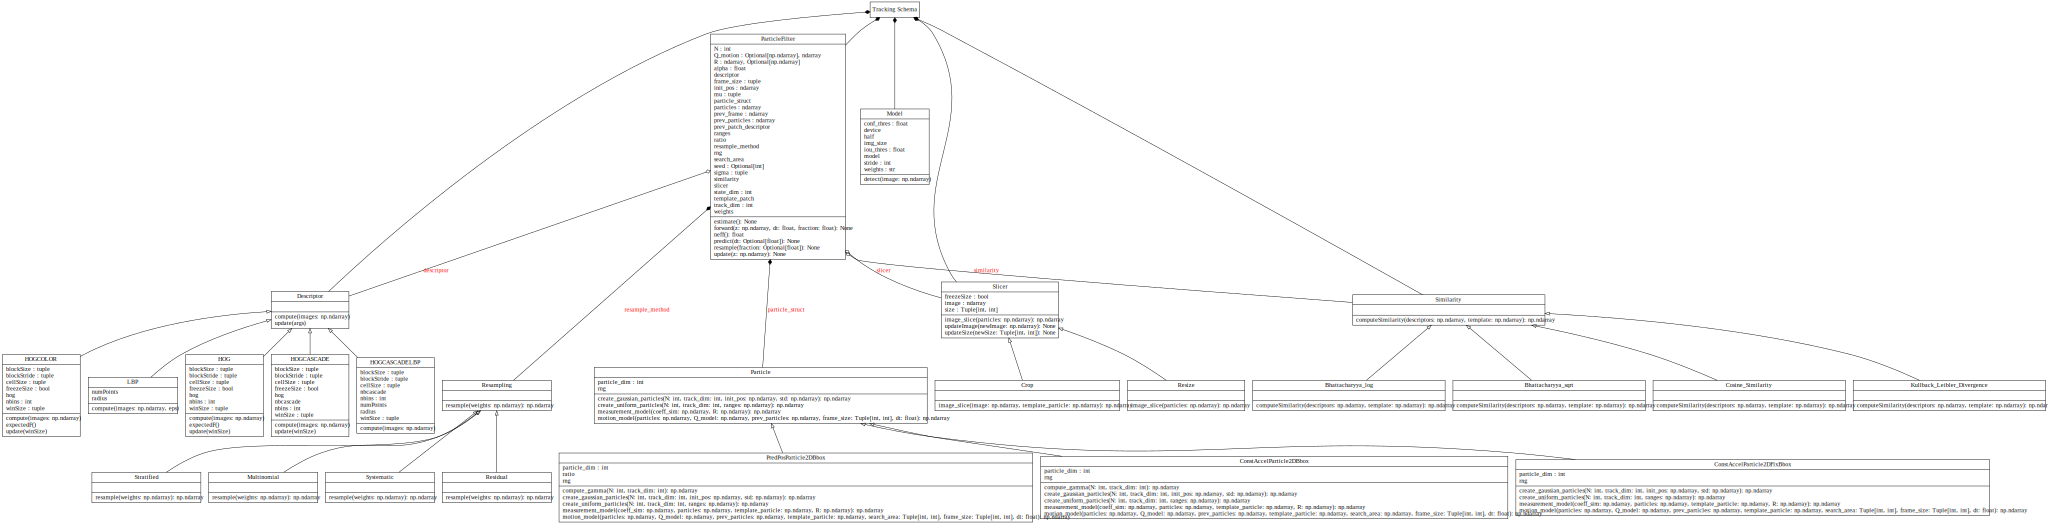
\includegraphics[scale=0.085]{classes.png}}}
\caption{Diagramme UML des classes.}
\label{fig:uml_diagram_classes}
\end{figure}
\FloatBarrier

\begin{figure}[!htbp]
\center
	\subfloat{{\includegraphics[scale=0.4]{usecase.png}}}
\caption{Diagramme UML de cas d'utilisation.}
\label{fig:uml_diagram_usecase}
\end{figure}
\FloatBarrier




\section{Structures de données}
Les structures de données principales du projet sont les tenseurs en tant que tableau multidimensionnel, pour ce faire, nous utilisons la librairie Numpy, qui permet de réaliser des opérations sur ces tableaux de façon optimisé.\\
Nous essayons de garder les données un maximum sous ce format, pour éviter les conversions et opérations qui pourraient ralentir le logiciel de suivi. C'est pour cela que la majorité des entrées des programmes réalisés demande des 'ndarray', qui est le type des tableaux Numpy.\\
\\
Les images prisent en entrée des programmes sont transformées en tableau Numpy, selon la convention de OpenCV, c'est-à-dire avec les couleurs au format BGR et la hauteur de l'image comme première dimension du tenseur, et la largeur de l'image comme seconde dimension.\\
\\
L'utilisateur du logiciel n'intervient qu'à un seul niveau dans le programme, le reste des entrées du logiciel est géré en interne afin de préserver au mieux l'intégrité des données traitées.\\
L'utilisateur peut uniquement donner des paramètres au logiciel lorsqu'il le lance, ces paramètres sont alors parser en différent arguments qui sont vérifiés par le programme, puis utilisés pour initialiser les différents module, afin de commencer le suivi d'une seiche.




\section{Statistiques}
Le projet compte un total de 25 classes réparties dans 10 scripts python (voir figure \ref{fig:uml_diagram_classes}).\\
Les scripts et classes de YOLOv7\cite{wang_yolov7_nodate} utilisés dans le projet ne sont pas comptés.\\
Le projet compte en tout 1576 lignes de code.\\
L'entièreté du projet est en accès libre sur github (\cite{pp2pf}).

\clearpage